% 
% Helios
% @author Pieter Maene <pieter.maene@student.kuleuven.be>
%

\chapter{Helios}
\label{chap:helios}

Het Helios verkiezingssysteem is een open-source project dat geleid wordt door Ben Adida.\cite{adida_helios} Het laat toe om online voter-verifiable verkiezingen te organiseren. Zoals vermeld in \ref{sec:ls:online_stemmen} kunnen online verkiezingen alleen gebruikt worden in een context waar dwang geen grote bedreiging vormt. Dit systeem werd vorig jaar door Robbert Coeckelbergh uitgebreid met threshold encryptie en gerangschikte verkiezingen.\cite{coeckelbergh_toepassing_en_uitbreiding_van_het_helios_online_verkiezingssysteem} 

\npar In dit hoofdstuk worden de belangrijkste cryptografische technieken uitgelegd die Helios gebruikt (\ref{sec:helios:cryptografische_technieken}). Daarna wordt de functionaliteit van de publieke delen van Helios besproken: het stemhokje (\ref{sec:helios:stemhokje}), het ballot tracking center (\ref{sec:helios:ballot_tracking_center}) en de controleapplicatie (\ref{sec:helios:controleapplicatie}).

\section{Cryptografische technieken}
\label{sec:helios:cryptografische_technieken}

Op het vlak van cryptografische technieken leunt Helios het dichtste aan bij Scratch \& Vote (\ref{sec:ls:scratch_and_vote}). Ook in Helios worden de stemmen ge\"encrypteerd. Na het aflopen van de stemming worden alle biljetten homomorf opgeteld. Tot slot wordt het resultaat gedecrypteerd. Alle ge\"encrypteerde stemmen worden ook online gepubliceerd, zodat iedereen kan verifi\"eren of het resultaat correct is.

\npar Het belangrijkste verschil is dat ElGamal gebruikt wordt in plaats van Paillier voor de homomorfe encryptie van de stemmen (\ref{sec:helios:elgamal} en \ref{sec:helios:homomorfe_encryptie}). Tot slot wordt de methode besproken waarop de sleutel verdeeld wordt tussen de trustees (\ref{sec:helios:threshold_encryptie}).

\subsection{ElGamal~\cite{elgamal_elgamal}}
\label{sec:helios:elgamal}

Het ElGamal \textit{cryptosystem} is een asymmetrisch schema dat gebaseerd is op het Diffie-Hellman protocol. Dit betekent dat een sleutelpaar met zowel een geheime als publieke sleutel nodig is. De publieke sleutel wordt gebruikt om de klaartekst te encrypteren. De decryptie kan alleen uitgevoerd worden met de geheime sleutel.

\npar Er wordt gewerkt in de groep $\mathbb{Z}_p$ waar $g$ de generator is. De geheime sleutel $sk$ wordt willekeurig gekozen binnen $\mathbb{Z}_{p-1}$. De publieke sleutel is dan ${pk} = g^{sk} \mod{p}$. De cijfertekst van een ElGamal encryptie bestaat uit twee delen: $c_1$ (\ref{eq:helios:elgamal_c1}) en $c_2$ (\ref{eq:helios:elgamal_c2}). In deze vergelijkingen is $m$ de klaartekst en $r$ opnieuw een willekeurig getal binnen $\mathbb{Z}_{p-1}$. $c_1$ en $r$ hebben respectievelijk de functie van tijdelijke publieke en private sleutel.\cite{preneel_cryptography_and_network_security}

\begin{align}
  \label{eq:helios:elgamal_c1} 
  c_1 & = g^r \mod{p} \\
  \label{eq:helios:elgamal_c2}
  c_2 & = m \cdot {pk}^r \mod{p}
\end{align}

\npar De cijfertekst kan dan gedecrypteerd worden volgens \ref{eq:helios:elgamal_m}.

\begin{equation}
  \label{eq:helios:elgamal_m}
  m = \frac{c_2}{c_1^{sk}} \mod{p}
\end{equation}

\subsection{Homomorfe encryptie}
\label{sec:helios:homomorfe_encryptie}

Bij homomorfe encryptie kan een specifieke operatie met de cijfertekst uitgevoerd worden. De resulterende cijfertekst is de encryptie van een bepaalde bewerking op de klaarteksten.\cite{wiki:homomorphic_encryption} Zo is het Paillier cryptosystem dat gebruikt wordt in Scratch \& Vote (\ref{sec:ls:scratch_and_vote}) homomorf onder $(\times, +)$. Dit betekent dat een vermenigvuldiging van de cijferteksten resulteert in een optelling van de klaarteksten.

\npar Het homomorfisme $(\times, +)$ kan in een verkiezingssysteem gebruikt worden om effici\"ent de stemmen op te tellen. De berekening van het resultaat kan immers gebeuren aan de hand van de cijferteksten. Er moet nu alleen een decryptie gebeuren om het uiteindelijke resultaat vrij te geven.

\npar Aan de hand van \ref{eq:helios:elgamal_c2} kan gezien worden dat ElGamal standaard homomorf is onder $(\times, \times)$. Zoals hiervoor besproken, is voor een verkiezingssysteem echter het homomorfisme $(\times, +)$ nodig. Dit kan gerealiseerd worden door de klaartekst ook in de exponent te plaatsen (\ref{eq:helios:elgamal_c2_homomorphic}).

\begin{equation}
  \label{eq:helios:elgamal_c2_homomorphic}
  c_2 = g^m \cdot {pk}^r \mod{p}
\end{equation}

\ref{eq:helios:elgamal_homomorphic} geeft het homomorfisme dat zo bekomen wordt.

\begin{equation}
  \label{eq:helios:elgamal_homomorphic}
  \begin{array}{lcl}
    \mathcal{E}(m_1) \cdot \mathcal{E}(m_2) &=& (g^{r_1}, g^{m_1} \cdot {pk}^{r_1}) \cdot (g^{r_2}, g^{m_2} \cdot {pk}^{r_2}) \\
      &=& (g^{r_1 + r_2}, g^{m_1 + m_2} \cdot {pk}^{r_1 + r_2}) \\
      &=& \mathcal{E}(m_1 + m_2)
  \end{array}
\end{equation}

\npar Omwille van het discreet logaritme probleem is het terugvinden van $m$ echter niet meer zo vanzelfsprekend.\cite{menezes_vanstone_oorschot_handbook_of_applied_cryptography} Dit kan alleen gedaan worden door $g^m \mod{p}$ te berekenen voor elke $m$ en vervolgens te zoeken welke hetzelfde is als de klaartekst van de decryptie.

\npar Scratch \& Vote (\ref{sec:ls:scratch_and_vote}) gebruikt multi-counters voor een stemming met meerdere kandidaten. Helios daarentegen encrypteert ieder mogelijk antwoord op een vraag afzonderlijk. Wanneer het antwoord gekozen wordt, is $m = 1$; anders wordt $m = 0$ gesteld.

\subsection{Threshold encryptie}
\label{sec:helios:threshold_encryptie}

Oorspronkelijk kon de publieke sleutel voor de verkiezing alleen berekend worden als het product van de afzonderlijke publieke sleutels van de \textit{trustees} (\ref{eq:helios:elgamal_c2_homomorphic_trustees}). Voor de decryptie moet iedere trustee zijn factor uit de noemer van \ref{eq:helios:elgamal_m_homomorphic_trustees} berekenen. Deze factoren worden in Helios de decryptiefactoren genoemd.

\begin{equation}
  \label{eq:helios:elgamal_c2_homomorphic_trustees}
  PK = \prod_{i=1}^n{{pk}_i} \mod{p}
\end{equation}

\begin{equation}
  \label{eq:helios:elgamal_m_homomorphic_trustees}
  g^m = \frac{c_2}{\prod_{i=1}^n{c_1^{{sk}_i}}} = \frac{c_2}{\prod_{i=1}^n{{df}_i}} \mod{p}
\end{equation}

\npar Een groot probleem hierbij is dat wanneer \'e\'en trustee zijn geheime sleutel verliest, het resultaat niet meer gedecrypteerd kan worden. Daarom werd threshold encryptie toegevoegd door Robbert Coeckelbergh.\cite{coeckelbergh_toepassing_en_uitbreiding_van_het_helios_online_verkiezingssysteem} Er kan nu een threshold schema gedefinieerd worden zodat slechts $k$ van de $n$ trustees hun decryptiefactor moeten berekenen.

\subsubsection{Secret Sharing}

De methode die ge\"implementeerd werd, is gebaseerd op Shamir's secret sharing.\cite{shamir_how_to_share_a_secret} Iedere trustee genereert eerst een veelterm van graad $k - 1$. Vervolgens stuurt hij elke trustee (ook zichzelf) een zogeheten \textit{share} van deze veelterm. Deze share is de waarde van de veelterm voor een punt $x$. Deze $x$-co\"ordinaat moet door iedereen gekend zijn, omdat het vereist is dat de shares die een trustee ontvangt van de anderen voor dezelfde waarde werden aangemaakt. Daarom wordt hiervoor binnen Helios het database ID van de trustee gebruikt. Dit is een uniek natuurlijk getal dat wordt opgehoogd telkens een nieuwe trustee aangemaakt wordt. Door \textit{zero-knowledge} bewijzen op te stellen, wordt heel dit proces verifiable. Hier wordt echter niet verder op ingegaan.

\npar Vervolgens moet de trustee de $n$ shares die hij zo ontvangt, optellen. Zo bekomt hij de $y$-co\"ordinaat die hoort bij zijn ID op een nieuwe veelterm, die de som is van de $n$ veeltermen die door de trustees gegenereerd werden. Deze waarde kan hij nu gebruiken als zijn geheime sleutel ${sk}$. Omdat ElGamal gebruikt wordt als encryptieschema, wordt zijn publieke sleutel ${pk} = g^{sk} \mod{p}$.

\npar Als geheime sleutel voor de verkiezing wordt nu de waarde voor $x = 0$ op de gemeenschappelijke veelterm genomen. Deze veelterm kan door Lagrange-interpolatie gereconstrueerd worden uit $k$ punten. Hiervoor worden de eerste $k$ trustees gebruikt (dat zijn deze met het laagste ID). Omdat alleen de publieke sleutels van de trustees beschikbaar zijn, wordt echter onmiddellijk de publieke sleutel voor de verkiezing berekend (\ref{eq:helios:threshold_encryption_public_key}).

\begin{align}
  \label{eq:helios:threshold_encryption_lagrange}
  \lambda_i(x) & = \prod_{j=1, j\not=i}^k{\frac{x - x_j}{x_i - x_j}} \\
  \label{eq:helios:threshold_encryption_polynomial}
  V(x) & = \sum_{i=1}^k{{sk}_i\lambda_i(x)}
\end{align}

\begin{align}
  \label{eq:helios:threshold_encryption_secret_key}
  SK & = V(0) = \sum_{i=1}^k{{sk}_i\lambda_i(0)} \\
  \label{eq:helios:threshold_encryption_public_key}
  PK & = g^{X} = \prod_{i=1}^k{{pk}_i^{\lambda_i(0)}} \mod{p}
\end{align}

\npar Om het resultaat te decrypteren, moet de geheime sleutel voor de verkiezing gebruikt worden (\ref{eq:helios:threshold_encryption_secret_key}). Het grote voordeel van threshold encryptie is dat het hier niet belangrijk is van welke $k$ trustees de decryptiefactoren en bijhorende Lagrange-interpolatie gebruikt worden.

\begin{equation}
  \label{eq:helios:threshold_encryption_m}
  g^m = \frac{c_2}{\prod_{i=1}^k{c_1^{{sk}_i\lambda_i(0)}}} = \frac{c_2}{\prod_{i=1}^k{{df}_i^{\lambda_i(0)}}} \mod{p}
\end{equation}

\subsubsection{Communicatiesleutels}
\label{sec:helios:communicatiesleutels}

Voordat iedere trustee zijn gegenereerde shares doorstuurt naar de andere trustees, worden deze ge\"encrypteerd en getekend. Hiervoor worden respectievelijk de publieke sleutel voor encryptie en de publieke sleutel voor tekenen van de andere trustee gebruikt. Dit geeft aanleiding tot twee nieuwe sleutelparen die de communicatiesleutels genoemd worden.

\section{Toepassing in Helios}

De cryptografische technieken van \ref{sec:helios:cryptografische_technieken} worden in Helios gebruikt om de stemmen te encrypteren (\ref{sec:helios:stemhokje}). Het Ballot Tracking Center is het publieke bulletin board uit Scratch \& Vote waarop alle kiezers en hun stem gepubliceerd worden (\ref{sec:helios:ballot_tracking_center}). De controleapplicatie (\ref{sec:helios:controleapplicatie}) kan gebruikt worden door de kiezer om na te gaan of het resultaat correct is.

\subsection{Stemhokje}
\label{sec:helios:stemhokje}

Het stemhokje staat volledig los van de rest van het systeem. Het is een applicatie die de kiezer kan gebruiken om zijn stem uit te brengen. Nadat hij zijn keuze gemaakt heeft, wordt deze ge\"encrypteerd met de publieke sleutel voor de verkiezing. Zoals besproken in \ref{sec:helios:cryptografische_technieken}, zal de cijfertekst bestaan uit twee delen (\ref{eq:helios:elgamal_c1} en \ref{eq:helios:elgamal_c2_homomorphic}). Wanneer threshold encryptie aanstaat, wordt de publieke sleutel zoals gedefinieerd door \ref{eq:helios:threshold_encryption_public_key} gebruikt; anders is het deze van \ref{eq:helios:elgamal_c2_homomorphic_trustees}. Daarnaast worden ook zero-knowledge bewijzen opgesteld voor de stem, maar hier wordt niet dieper op ingegaan.

\npar Het encryptieproces is in JavaScript ge\"implementeerd en vindt dus volledig plaats in de browser van de kiezer. Zijn stem zal dan ook nooit onge\"encrypteerd op de server toekomen. Alle informatie over de verkiezing kan eenvoudig opgevraagd worden. De kiezer zou dus ook zijn eigen software kunnen gebruiken om zijn stem te encrypteren.

\npar Aan elke ge\"encrypteerde stem wordt een \textit{smart ballot tracker} toegekend. Dit is een fingerprint die de stem identificeert (\ref{sec:sf:fingerprints}). Aan de hand daarvan kan de kiezer zijn stem volgen doorheen het systeem en kan hij verifi\"eren of ze niet aangepast is.

\subsection{Ballot Tracking Center}
\label{sec:helios:ballot_tracking_center}

Net zoals bij Scratch \& Vote (\ref{sec:ls:scratch_and_vote}) worden de uitgebrachte stemmen gepubliceerd. In het ballot tracking center kan een lijst met alle kiezers teruggevonden worden. Bij een publieke verkiezing kan iedereen deze opvragen, bij een private alleen de geregistreerde kiezers. Standaard staan hier gewoon de namen van de kiezers, maar de beheerder kan ervoor kiezen om aliassen te gebruiken in de plaats.

\npar Van zodra een kiezer zijn stem uitgebracht heeft, kan deze door iedereen bekeken worden (\ref{fig:helios:cast_vote}). Dit is nodig omdat zo het resultaat van de verkiezing gecontroleerd kan worden (\ref{sec:helios:controleapplicatie}). Al deze informatie kan ook opgevraagd worden als JSON, zodat de applicatie ze eenvoudiger kan verwerken. Een derde partij zou deze functionaliteit dus ook zelf kunnen implementeren.

\begin{figure}
  \center{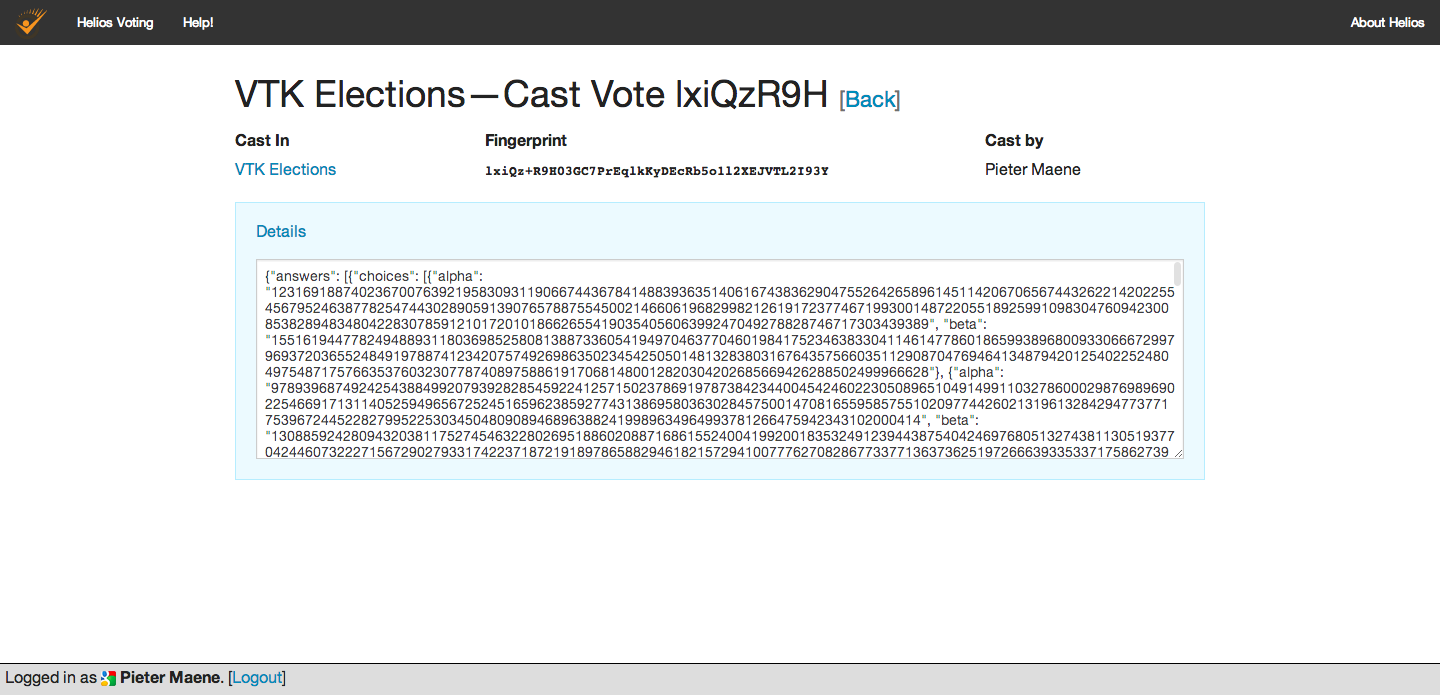
\includegraphics[width=0.9\linewidth]{helios/cast_vote.png}}
  \caption{Uitgebrachte stem}
  \label{fig:helios:cast_vote}
\end{figure}

\subsection{Controleapplicatie}
\label{sec:helios:controleapplicatie}

Net zoals het stemhokje is de controleapplicatie onafhankelijk en draait ze lokaal in de browser van de gebruiker. Ze kan gebruikt worden om het resultaat van de verkiezing te controleren. Alle ruwe data wordt gedownload van de server, waarna de nodige berekeningen lokaal worden uitgevoerd.
